
De impact analyse is uitgevoerd op basis van een methodiek gebruikt door \textcite{fema}, daarin wordt omschreven: "Hazard identification and risk assessment provides the factual basis for activities proposed in the strategy portion of a hazard mitigation plan. An effective risk assessment informs proposed actions by focusing attention and resources on the greatest risks.". 

De resultaten zijn verwerkt in deelvraag 3 in \ref{sec:deelvraag3}.

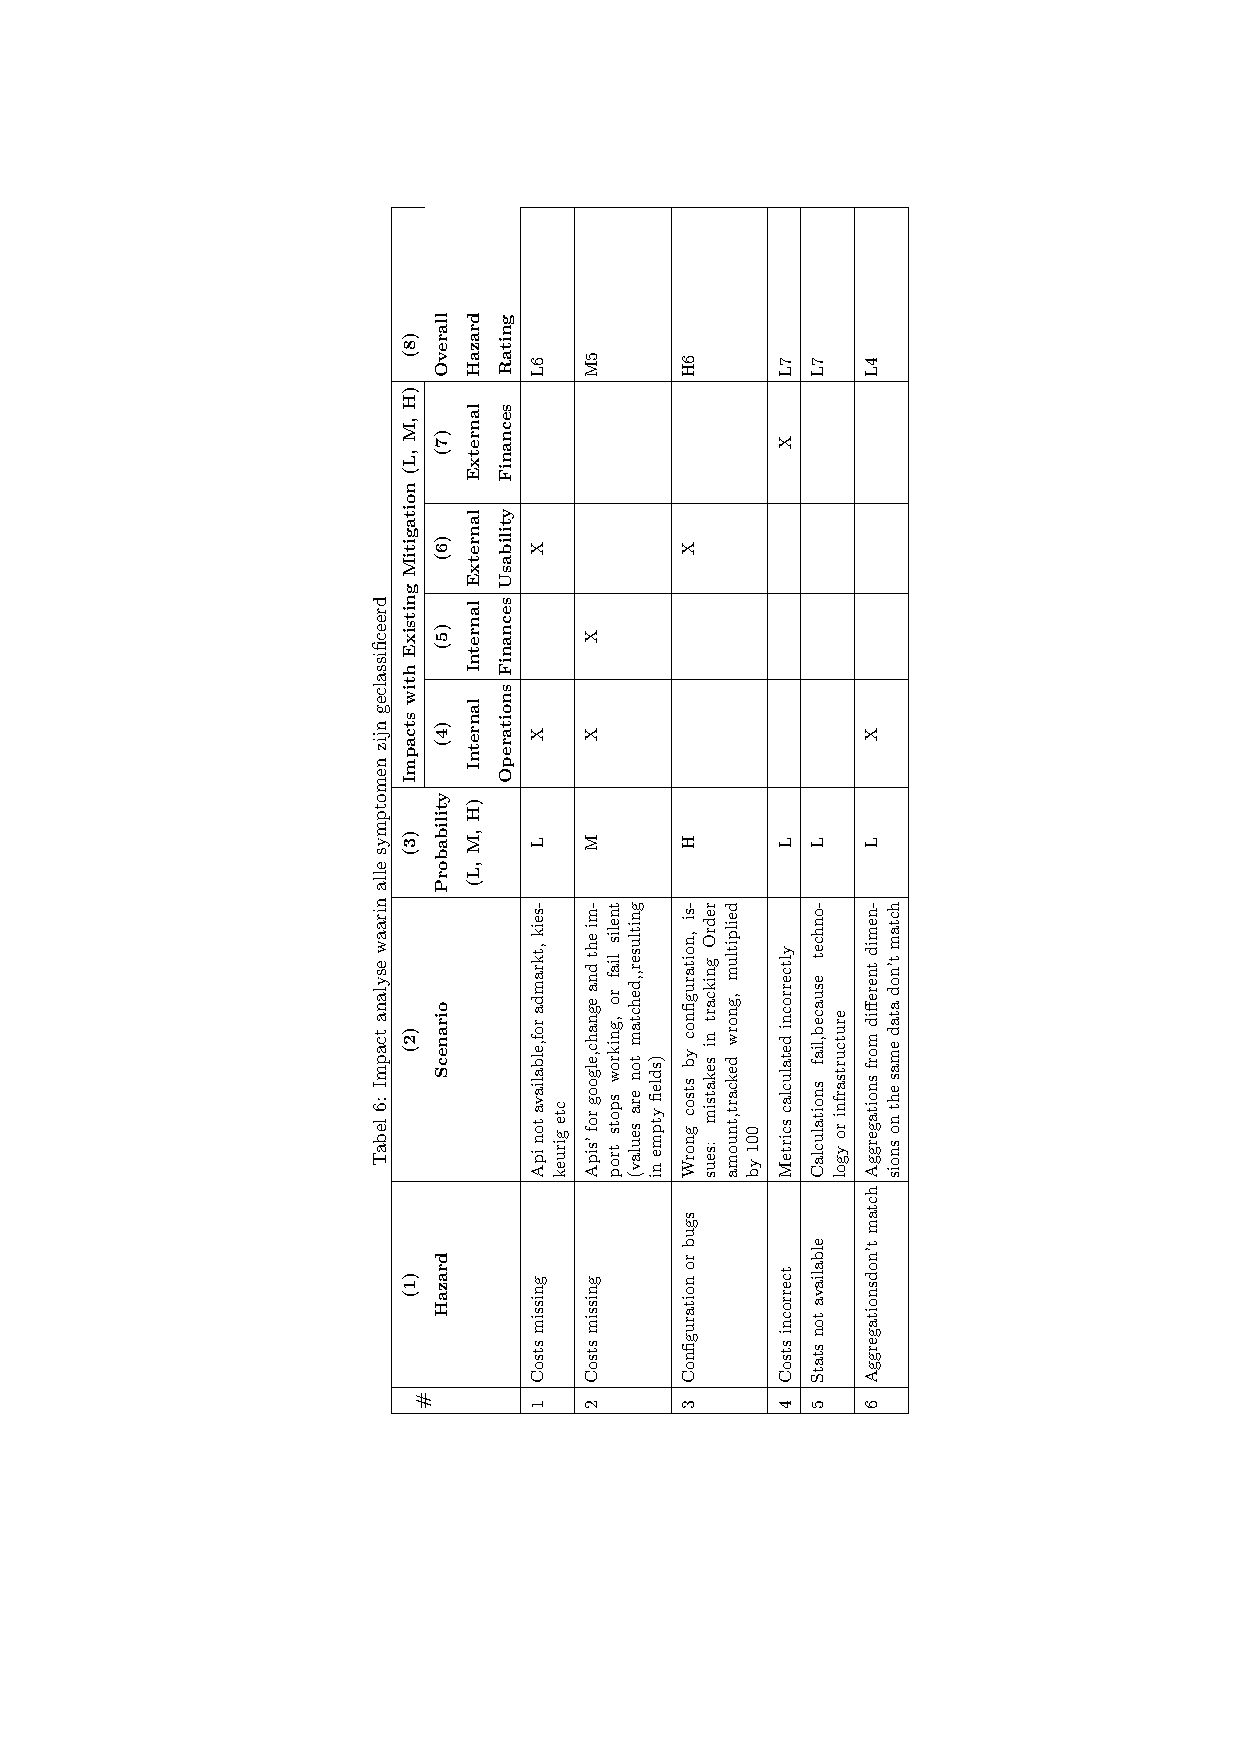
\includepdf[pages={1,2}]{appendix/impact-analyse-A.pdf}